\section{Appendix II: Previous versions of analysis patterns} \label{appendix2}
Below is a previous version of analysis patterns. It was decided that keeping track of \emph{balance}

The first analysis patterns which seem appropriate are the \emph{Account}
pattern, used to create the \emph{Category} entity class, and the
\emph{Quantity} pattern for the \emph{Amount} entity class
(\cite[][Sections~6.1~\&~3.1]{fowler1997analysis}):
\begin{figure}[ht!]
  \begin{center}
    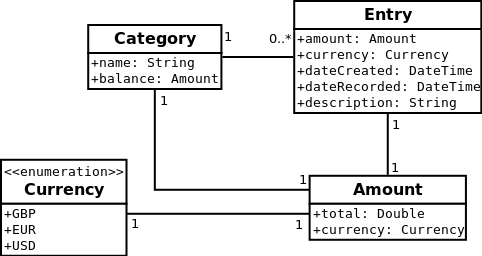
\includegraphics[width=11cm]{./contents/img/Class_Diagram_-_Categories_and_Amount.png}
  \end{center}
  \caption{}
  \label{fig:ClassDiagram.CategoriesAndAmount}
\end{figure}
\FloatBarrier

As implied by the diagram above, the \emph{Category} class will be associated
with instances of the \emph{Entry} class, and will keep track of the balance
made up of the sum of \emph{Amount}'s of each entry. This is done so that the
only way to change the total of a category is by adding positive or negative
entries to it -- for example, to indicate a credit to a category, a negative
entry can be added to it.

Another design choice which can be observed in Figure
\ref{fig:ClassDiagram.CategoriesAndAmount} is that the \emph{Amount} class also
possesses an attribute for currency. This has been designed so as to allow for
the possibility of extending the design to keep track of transactions in
multiple currencies, although it was not a specific requirement. Initially,
there will only be a single default currency which shall be set at runtime.

The next step is to provide a way for these entries to be added to categories.
For this to happen, there needs to be a constraint to ensure that double entry
happens every time a change needs to be made to a category. One of the ways to
achieve this is to apply the \emph{Transaction} pattern
(\cite[][Section~6.2]{fowler1997analysis}):
\begin{figure}[ht!]
  \begin{center}
    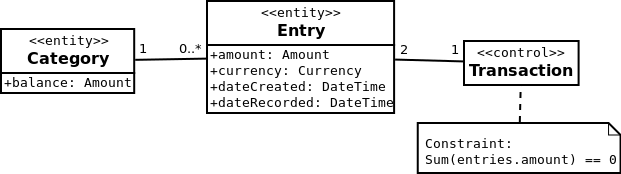
\includegraphics[width=14cm]{./contents/img/Class_Diagram_-_Transaction.png}
  \end{center}
\end{figure}
\FloatBarrier

After having determined the analysis patterns which shall be employed, it makes
sense to dive into a deeper analysis of the use cases described in Chapter
\ref{sec:Requirements}. At this point the objective will be to start modelling
classes based on concepts or things found in the problem domain. This will be
done in the following subsections.
